
% This LaTeX was auto-generated from MATLAB code.
% To make changes, update the MATLAB code and republish this document.

\documentclass{article}
\usepackage{graphicx}
\usepackage{color}

\sloppy
\definecolor{lightgray}{gray}{0.5}
\setlength{\parindent}{0pt}

\begin{document}

    
    
\subsection*{Contents}

\begin{itemize}
\setlength{\itemsep}{-1ex}
   \item Initialization and model definition
   \item Generate system matrixes for linear model
   \item Solve QP problem with linear model
   \item Extract control inputs and states
   \item Plotting
\end{itemize}
\begin{verbatim}
% TTK4135 - Helicopter lab
% Hints/template for problem 2.
% Updated spring 2017, Andreas L. Fl?ten
\end{verbatim}


\subsection*{Initialization and model definition}

\begin{verbatim}
code22; % NB: Change this to the init file corresponding to your helicopter
delta_t	= 0.25; % sampling time

% Discrete time system model. x = [lambda r p p_dot]'
A1 = A;
B1 = B;

% Number of states and inputs
mx = size(A1,2); % Number of states (number of columns in A)
mu = size(B1,2); % Number of inputs(number of columns in B)

% Initial values
x1_0 = pi;                               % Lambda
x2_0 = 0;                               % r
x3_0 = 0;                               % p
x4_0 = 0;                               % p_dot
x0 = [x1_0 x2_0 x3_0 x4_0]';          % Initial values

% Time horizon and initialization
N  = 100;                                % Time horizon for states
M  = N;                                 % Time horizon for inputs
z  = zeros(N*mx+M*mu,1);                % Initialize z for the whole horizon
z0 = z;                                 % Initial value for optimization

% Bounds
ul 	    = -30*pi/180;                   % Lower bound on control -- u1
uu 	    = 30*pi/180;                    % Upper bound on control -- u1

xl      = -Inf*ones(mx,1);              % Lower bound on states (no bound)
xu      = Inf*ones(mx,1);               % Upper bound on states (no bound)
xl(3)   = ul;                           % Lower bound on state x3
xu(3)   = uu;                           % Upper bound on state x3

% Generate constraints on measurements and inputs
[vlb,vub]       = hints_genbegr2(N,M,xl,xu,ul,uu);      % hint: genbegr2
vlb(N*mx+M*mu)  = 0;                                    % We want the last input to be zero
vub(N*mx+M*mu)  = 0;                                    % We want the last input to be zero

% Generate the matrix Q and the vector c (objecitve function weights in the QP problem)
Q1 = zeros(mx,mx);
Q1(1,1) = 1;                            % Weight on state x1
Q1(2,2) = 0;                            % Weight on state x2
Q1(3,3) = 0;                            % Weight on state x3
Q1(4,4) = 0;                            % Weight on state x4
P1 = 1;                                 % Weight on input
Q = 2*hints_genq2(Q1,P1,N,M,mu);        % Generate Q
c = zeros(N*mx+M*mu,1);                 % Generate c
\end{verbatim}


\subsection*{Generate system matrixes for linear model}

\begin{verbatim}
Aeq = hints_gena2(A1,B1,N,mx,mu);           % Generate A, hint: gena2
beq = zeros(mx*N, 1);                       % Generate b
beq(1:mx) = A1*x0;                          % Initial value

%User input
%G = hints_blkdiag(Q,c);
\end{verbatim}


\subsection*{Solve QP problem with linear model}

\begin{verbatim}
tic
[z,lambda] = quadprog(Q,c,[],[],Aeq,beq,vlb,vub); % hint: quadprog
t1=toc;

% Calculate objective value
phi1 = 0.0;
PhiOut = zeros(N*mx+M*mu,1);
for i=1:N*mx+M*mu
  phi1=phi1+Q(i,i)*z(i)*z(i);
  PhiOut(i) = phi1;
end
\end{verbatim}

        \color{lightgray} \begin{verbatim}
Minimum found that satisfies the constraints.

Optimization completed because the objective function is non-decreasing in 
feasible directions, to within the default value of the optimality tolerance,
and constraints are satisfied to within the default value of the constraint tolerance.



\end{verbatim} \color{black}
    

\subsection*{Extract control inputs and states}

\begin{verbatim}
u  = [z(N*mx+1:N*mx+M*mu);z(N*mx+M*mu)]; % Control input from solution

x1 = [x0(1);z(1:mx:N*mx)];              % State x1 from solution
x2 = [x0(2);z(2:mx:N*mx)];              % State x2 from solution
x3 = [x0(3);z(3:mx:N*mx)];              % State x3 from solution
x4 = [x0(4);z(4:mx:N*mx)];              % State x4 from solution

num_variables = 5/delta_t;
zero_padding = zeros(num_variables,1);
unit_padding  = ones(num_variables,1);

u   = [zero_padding; u; zero_padding];
x1  = [pi*unit_padding; x1; zero_padding];
x2  = [zero_padding; x2; zero_padding];
x3  = [zero_padding; x3; zero_padding];
x4  = [zero_padding; x4; zero_padding];
\end{verbatim}


\subsection*{Plotting}

\begin{verbatim}
t = 0:delta_t:delta_t*(length(u)-1);

figure(23)
subplot(511)
stairs(t,u),grid
ylabel('u')
subplot(512)
plot(t,x1,'m',t,x1,'r'),grid
ylabel('lambda')
subplot(513)
plot(t,x2,'m',t,x2','r'),grid
ylabel('r')
subplot(514)
plot(t,x3,'m',t,x3,'r'),grid
ylabel('p')
subplot(515)
plot(t,x4,'m',t,x4','r'),grid
xlabel('tid (s)'),ylabel('pdot')


ut = [t' u];
\end{verbatim}

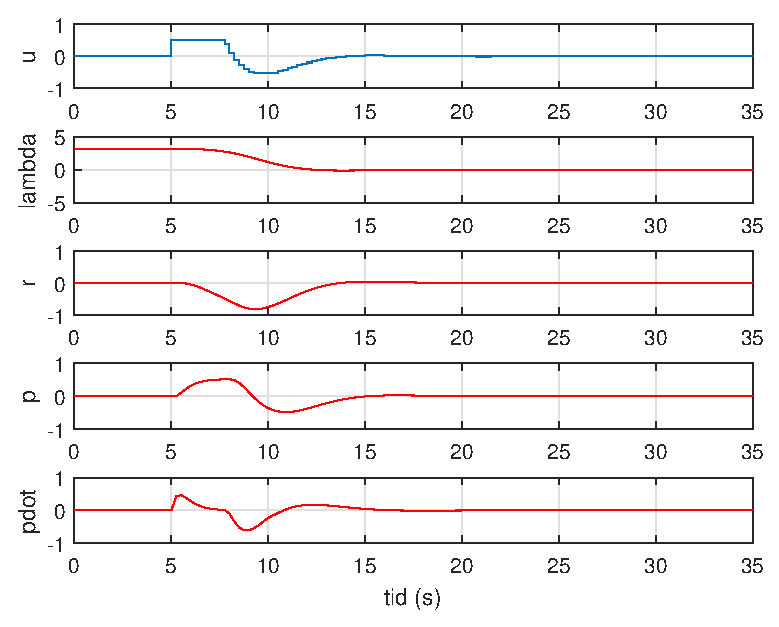
\includegraphics [width=4in]{code23_01.eps}



\end{document}
    
